\section{\texorpdfstring{Latinské čtverce}{Latinské čtverce}}
\vspace{5mm}
\large

\begin{definition}
	Latinský obdélník je matice $L \in X^{k \times n}$. Taková, že prvky se neopakuji ani ve sloupcích ani v řádcích.
	Kde $X$ je n-prvková množina. Typický $\{ 1, ..., n \} := [n]$.

	Na řádky lze nahlížet jako na permutace.
\end{definition}

\begin{theorem}[Latinské čtverce]
	Každý Latinský obdélník řádu $k \times n$ lze doplnit na Latinský čtverec řadu $n \times n$.
\end{theorem}
\begin{proof}
	Dokážeme přidaní nových řádků v závislostí na již existujících řádcích.

	V k-tem kroků se podíváme na j-tý sloupec.
	Nechť $M_j$ bude množina kandidátů které můžeme dat na j-tou pozici v novém řádku.
	\[ M_j = [n]\setminus \{ L_{ij}: i = 1, 2, ... , k \} \]

	Teď musíme z množin $M_j$ vzít po 2 různé prvky.
	Jinými slovy, hledáme Systém různých reprezentantů - SRR pro $\{ M_j \}_1^n$.

	Sestavíme graf, kde vrcholy jsou množiny $M_j$ a prvky z $[n]$.
	\[ (l, M_j) \in E \iff l \in M_j \]

	Pak tento bipartitní graf je $(n - k)$-regulární.
	Protože $\forall x$ je v $(n - k)$ množinách $M_j$.

	Dle Hallové věty, v takovém grafu existuje perfektní párovaní, které určuje SRR.
\end{proof}

\begin{consequence}
	Latinských čtverců řádu $n$ je $\bigO(n!)$.
\end{consequence}
\begin{proof}
	BUNO: v prvním řádku je $\{ 1, 2, ..., n \}$.
	Jinak můžeme vhodně přejmenovat prvky.

	V druhém řádku musí být permutace $[n]$ bez pevných bodů.
	Z \emph{problému šatnářky} takových permutaci je
	\[ \frac{n!}{e} \]
	Pak dle věty každý obdélník lze doplnit na čtverec.
\end{proof}

\begin{definition}
	Latinský čtverce jsou kolmé %todo

	Taky lze definovat ortogonalitu nad různými množiny.
\end{definition}

\begin{notation}
	$NOLČ(n)$ značíme největší počet navzájem ortogonálních Latinských čtverců řádu $n$.
\end{notation}

\begin{theorem}[Horní odhad NOLČ]
	\[\forall n \in \N, n > 1: NOLČ(n) \leq n - 1 \]
\end{theorem}
\begin{proof}
	Nechť
	\[L^1, ..., L^t \in \{ 1, ..., n \}^{n \times n}, \forall i \neq j: L^i \perp L^j \]

	BUNO: přejmenujeme prvky v každém LČ tak, aby v prvním řádku bylo $\{ 1, 2, ..., n \}$.
	Takto vyrobíme LČ $L^{1 \prime}, ..., L^{t \prime}$.

	Tvrdíme ale, že ortogonalita je zachovaná.
	Obecně pro libovolná permutace $\pi$ aplikovaná ne jeden z dvojice ortogonálních LČ zachovává ortogonalitu.

	Pak na pozici $(2,1)$ nemůže být 1.
	Pokud tam ale bude nějaké písmeno $a$, tak čtverce nebudou ortogonální, protože všechny dvojice $(i, i)$ máme v prvním řádku.
	Z toho na pozice $(2,1)$ můžou být prvky $\{ 2, ..., n \}$ po 2 různé.
	Takže $NOLČ(n) \leq n - 1 $.
\end{proof}

Kdy máme extremální řešení?

\begin{theorem}[Extremální NOLČ a KPR]
	\[ NOLČ(n) = n - 1 \iff \exists KPR(n) \]
	Z předchozí přednášky platí pro mocniny prvočísla.
\end{theorem}
\begin{proof}
	$KRP \Rightarrow LČ$. Sestavíme nevlastní přímku A, svislé a vodorovné přímky.
	Dal přímky spojující A a průniky svislých a vodorovných přímek budou určovat LČ.
	\[ L^{\alpha}_{i,j} = \beta \iff x_{i,j} \in k_{\alpha, \beta} \]

	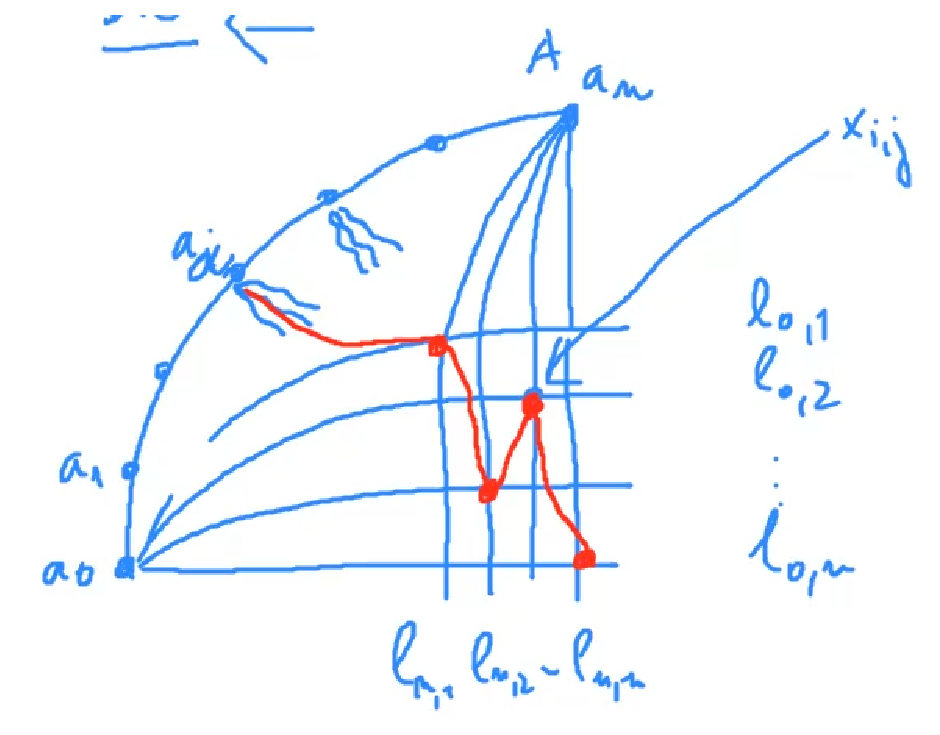
\includegraphics[scale=0.3]{lc_0.eps}

	Pak písmena v LČ odpovídající červené přímce budou:

	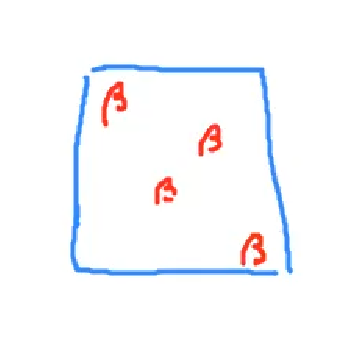
\includegraphics[scale=0.4]{lc_1.eps}

	Z axiomu KPR svislé, vodorovné a přímky procházející body $a_{\alpha}$ se protínají právě v 1 bodě.
	Takže písmena se neopakuji v rádcích a sloupcích.

	Jsou $\perp$ protože
	\[ \forall \beta, \beta^{\prime} \exists ! (i, j): L^{\alpha}_{i, j} = \beta \land L^{\gamma}_{i,j} = \beta^{\prime} \]
	Protože přímky se nemůžou protínat na nevlastní přímce A, takže se protínají uvnitř šachovnice.
	\[ \exists ! x_{i, j} \in l_{\alpha, \beta} \cap l_{\gamma, \beta^{\prime}} \]

	$LČ \Rightarrow KPR$. Nechť máme LČ
	\[ L^{\alpha}, \alpha \in \{ 1, 2, ... ,n - 1 \} \]
	Sestavíme nevlastní, svislé a vodorovné přímky.

	Šikmé přímky vytvoříme dle:
	\[ L^{\alpha}_{i,j} = \beta \iff x_{i,j} \in k_{\alpha, \beta} \]

	Ověříme axiomy:
	\begin{itemize}
		\item $A_1$. Přímky ze stejného svazku šikmých přímek se protínají v nevlastním bodě.
			Vodorovné a svislé se protínají v šachovnici.

			Šikmé vs svislé a Vodorovné vs svislé se protínají protože průniky jsou určené LČ.
			2 Šikmé přímky se protínají právě v 1 bodě protože čtverce jsou $\perp$.
		\item $A_3$. Plyne z toho, že $n \geq 2$.
		\item $A_2$. Spočítáme 2ma způsoby \# 3jic.
			\[ T = |\{ ((x,y), l): x \ne y \in X, l \in L, x,y \in l \}| \]
			Máme $(n^2 + n + 1)$ přímek, na každé z nich je $(n + 1)$ bodů. Pak
			\[ T = (n^2 + n + 1) \binom{n + 1}{2} \]
			Na druhou stranu, máme $(n^2 + n + 1)$ bodů. Každou 2ci prochází nejvýše 1 přímka.
			\[ T \leq 1 \cdot \binom{n^2 + n + 1}{2} \]
			Dohromady
			\[ (n^2 + n + 1) \binom{n + 1}{2} \leq \binom{n^2 + n + 1}{2} \]
			Po roznásobení dostaneme stejná čísla na obou stranách, což může nastat pouze v případě že každou 2cí bodů prochází \emph{právě 1} přímka.
	\end{itemize}
\end{proof}

\begin{definition}
	Ortogonální tabulka %todo prednaska 2 od 43:00
\end{definition}

\begin{theorem}[Ortogonální tabulka a NOLČ]
	\[ \forall n,d \in \N \exists OA(n, d) \iff NOLČ(n) \geq d - 2 \]
\end{theorem}
\begin{proof}
	%todo
\end{proof}

\begin{theorem}[Tenz produkt Ortogonálních tabulek]
	\[ \forall n,m,d \in \N \ \exists OA(n, d) \land OA(m, d) \Rightarrow \exists OA(mn, d) \]
\end{theorem}
\begin{proof}
	%todo
\end{proof}

\begin{theorem}[Dolní odhad NOLČ]
	Nechť $n = \prod_1^k p_i^{r_i}$ je faktorizace $n$. Pak
	\[ NOLČ(n) \geq \min_{i = 1}^k \{ p_i^{r_i} - 1 \}  \]
\end{theorem}
\begin{proof}
	%todo
\end{proof}

\begin{consequence}
	\[ \forall n \in \N, n > 2 \land n \neg \equiv 2 \mod 4: NOLČ(n) \geq 2 \]
\end{consequence}

\begin{lemma}
	\[ \exists OA(m, 4) \Rightarrow \exists OA(3m + 1, 4) \]
\end{lemma}

\begin{theorem}[Dolní odhad NOLČ - 2]
	\[ \forall k > 0: NOLČ(12 k + 10) \geq 2 \]
\end{theorem}
\begin{proof}
	%todo
\end{proof}
